%% bare_conf.tex
%% V1.3


% Note that the a4paper option is mainly intended so that authors in
% countries using A4 can easily print to A4 and see how their papers will
% look in print - the typesetting of the document will not typically be
% affected with changes in paper size (but the bottom and side margins will).
% Use the testflow package mentioned above to verify correct handling of
% both paper sizes by the user's LaTeX system.
%
% Also note that the "draftcls" or "draftclsnofoot", not "draft", option
% should be used if it is desired that the figures are to be displayed in
% draft mode.
%
\documentclass[a4paper,conference]{IEEEtran}


% *** CITATION PACKAGES ***
%
\usepackage{cite}
% cite.sty was written by Donald Arseneau
% V1.6 and later of IEEEtran pre-defines the format of the cite.sty package
% \cite{} output to follow that of IEEE. Loading the cite package will
% result in citation numbers being automatically sorted and properly
% "compressed/ranged". e.g., [1], [9], [2], [7], [5], [6] without using
% cite.sty will become [1], [2], [5]--[7], [9] using cite.sty. cite.sty's
% \cite will automatically add leading space, if needed. Use cite.sty's
% noadjust option (cite.sty V3.8 and later) if you want to turn this off.
% cite.sty is already installed on most LaTeX systems. Be sure and use
% version 4.0 (2003-05-27) and later if using hyperref.sty. cite.sty does
% not currently provide for hyperlinked citations.
% The latest version can be obtained at:
% http://www.ctan.org/tex-archive/macros/latex/contrib/cite/
% The documentation is contained in the cite.sty file itself.



% *** GRAPHICS RELATED PACKAGES ***
%
\ifCLASSINFOpdf
   \usepackage[pdftex]{graphicx}
  % declare the path(s) where your graphic files are
   \graphicspath{{./}}
  % and their extensions so you won't have to specify these with
  % every instance of \includegraphics
  \DeclareGraphicsExtensions{.pdf,.jpeg,.png}
\else
  % or other class option (dvipsone, dvipdf, if not using dvips). graphicx
  % will default to the driver specified in the system graphics.cfg if no
  % driver is specified.
  % \usepackage[dvips]{graphicx}
  % declare the path(s) where your graphic files are
  % \graphicspath{{../eps/}}
  % and their extensions so you won't have to specify these with
  % every instance of \includegraphics
  % \DeclareGraphicsExtensions{.eps}
\fi




\usepackage[cmex10]{amsmath}



\usepackage{algorithmic}




% *** ALIGNMENT PACKAGES ***
%
\usepackage{array}


\usepackage{mdwmath}
\usepackage{mdwtab}




% *** SUBFIGURE PACKAGES ***
\usepackage[tight,footnotesize]{subfigure}
% subfigure.sty was written by Steven Douglas Cochran. This package makes it
% easy to put subfigures in your figures. e.g., "Figure 1a and 1b". For IEEE
% work, it is a good idea to load it with the tight package option to reduce
% the amount of white space around the subfigures. subfigure.sty is already
% installed on most LaTeX systems. The latest version and documentation can
% be obtained at:
% http://www.ctan.org/tex-archive/obsolete/macros/latex/contrib/subfigure/
% subfigure.sty has been superceeded by subfig.sty.



\usepackage[caption=false]{caption}
\usepackage[font=footnotesize]{subfig}
% subfig.sty, also written by Steven Douglas Cochran, is the modern
% replacement for subfigure.sty. However, subfig.sty requires and
% automatically loads Axel Sommerfeldt's caption.sty which will override
% IEEEtran.cls handling of captions and this will result in nonIEEE style
% figure/table captions. To prevent this problem, be sure and preload
% caption.sty with its "caption=false" package option. This is will preserve
% IEEEtran.cls handing of captions. Version 1.3 (2005/06/28) and later 
% (recommended due to many improvements over 1.2) of subfig.sty supports
% the caption=false option directly:
%\usepackage[caption=false,font=footnotesize]{subfig}
%
% The latest version and documentation can be obtained at:
% http://www.ctan.org/tex-archive/macros/latex/contrib/subfig/
% The latest version and documentation of caption.sty can be obtained at:
% http://www.ctan.org/tex-archive/macros/latex/contrib/caption/




% *** FLOAT PACKAGES ***
%
\usepackage{fixltx2e}
% fixltx2e, the successor to the earlier fix2col.sty, was written by
% Frank Mittelbach and David Carlisle. This package corrects a few problems
% in the LaTeX2e kernel, the most notable of which is that in current
% LaTeX2e releases, the ordering of single and double column floats is not
% guaranteed to be preserved. Thus, an unpatched LaTeX2e can allow a
% single column figure to be placed prior to an earlier double column
% figure. The latest version and documentation can be found at:
% http://www.ctan.org/tex-archive/macros/latex/base/



%\usepackage{stfloats}
% stfloats.sty was written by Sigitas Tolusis. This package gives LaTeX2e
% the ability to do double column floats at the bottom of the page as well
% as the top. (e.g., "\begin{figure*}[!b]" is not normally possible in
% LaTeX2e). It also provides a command:
%\fnbelowfloat
% to enable the placement of footnotes below bottom floats (the standard
% LaTeX2e kernel puts them above bottom floats). This is an invasive package
% which rewrites many portions of the LaTeX2e float routines. It may not work
% with other packages that modify the LaTeX2e float routines. The latest
% version and documentation can be obtained at:
% http://www.ctan.org/tex-archive/macros/latex/contrib/sttools/
% Documentation is contained in the stfloats.sty comments as well as in the
% presfull.pdf file. Do not use the stfloats baselinefloat ability as IEEE
% does not allow \baselineskip to stretch. Authors submitting work to the
% IEEE should note that IEEE rarely uses double column equations and
% that authors should try to avoid such use. Do not be tempted to use the
% cuted.sty or midfloat.sty packages (also by Sigitas Tolusis) as IEEE does
% not format its papers in such ways.





% *** PDF, URL AND HYPERLINK PACKAGES ***
%
%\usepackage{url}
% url.sty was written by Donald Arseneau. It provides better support for
% handling and breaking URLs. url.sty is already installed on most LaTeX
% systems. The latest version can be obtained at:
% http://www.ctan.org/tex-archive/macros/latex/contrib/misc/
% Read the url.sty source comments for usage information. Basically,
% \url{my_url_here}.



% *** Do not adjust lengths that control margins, column widths, etc. ***
% *** Do not use packages that alter fonts (such as pslatex).         ***
% There should be no need to do such things with IEEEtran.cls V1.6 and later.
% (Unless specifically asked to do so by the journal or conference you plan
% to submit to, of course. )


% correct bad hyphenation here
\hyphenation{op-tical net-works semi-conduc-tor}


\begin{document}
%
% paper title
% can use linebreaks \\ within to get better formatting as desired
\title{Random Access Mechanisms for \\ DNA Storage Systems}


% author names and affiliations
% use a multiple column layout for up to three different
% affiliations
\author{\IEEEauthorblockN{Ryan Quinn Ford}
\IEEEauthorblockA{Philipps-University Marburg, Germany \\
Department of Mathematics and Computer Science, Distributed Systems Group \\
Email: ford@informatik.uni-marburg.de
}}

% conference papers do not typically use \thanks and this command
% is locked out in conference mode. If really needed, such as for
% the acknowledgment of grants, issue a \IEEEoverridecommandlockouts
% after \documentclass

% for over three affiliations, or if they all won't fit within the width
% of the page, use this alternative format:
% 
%\author{\IEEEauthorblockN{Michael Shell\IEEEauthorrefmark{1},
%Homer Simpson\IEEEauthorrefmark{2},
%James Kirk\IEEEauthorrefmark{3}, 
%Montgomery Scott\IEEEauthorrefmark{3} and
%Eldon Tyrell\IEEEauthorrefmark{4}}
%\IEEEauthorblockA{\IEEEauthorrefmark{1}School of Electrical and Computer Engineering\\
%Georgia Institute of Technology,
%Atlanta, Georgia 30332--0250\\ Email: see http://www.michaelshell.org/contact.html}
%\IEEEauthorblockA{\IEEEauthorrefmark{2}Twentieth Century Fox, Springfield, USA\\
%Email: homer@thesimpsons.com}
%\IEEEauthorblockA{\IEEEauthorrefmark{3}Starfleet Academy, San Francisco, California 96678-2391\\
%Telephone: (800) 555--1212, Fax: (888) 555--1212}
%\IEEEauthorblockA{\IEEEauthorrefmark{4}Tyrell Inc., 123 Replicant Street, Los Angeles, California 90210--4321}}




% use for special paper notices
%\IEEEspecialpapernotice{(Invited Paper)}




% make the title area
\maketitle


\begin{abstract}
%\boldmath
With the global amount of data growing at a speed that current storage technologies cannot hold pace with, researchers have looked to DNA for a novel storage solution. DNA provides an unprecedented data density and long-term durability, which is now being actualized for data storage thanks to ever-decreasing sequencing costs. However, due to very low read speeds and delicate conditions, it is of significant importance to find ways to more efficiently randomly access data in a DNA store, e.g., retrieving single files from a DNA database. In this paper, three recent breakthroughs in techniques for random access in DNA storage and their capabilities and outlook regarding scalability and error correction/detection are presented. In addition, the current limitations that face these techniques and what areas they open up to future research are discussed.
\end{abstract}
% IEEEtran.cls defaults to using nonbold math in the Abstract.
% This preserves the distinction between vectors and scalars. However,
% if the conference you are submitting to favors bold math in the abstract,
% then you can use LaTeX's standard command \boldmath at the very start
% of the abstract to achieve this. Many IEEE journals/conferences frown on
% math in the abstract anyway.

% no keywords




% For peer review papers, you can put extra information on the cover
% page as needed:
% \ifCLASSOPTIONpeerreview
% \begin{center} \bfseries EDICS Category: 3-BBND \end{center}
% \fi
%
% For peerreview papers, this IEEEtran command inserts a page break and
% creates the second title. It will be ignored for other modes.
\IEEEpeerreviewmaketitle


\section{Introduction}

\subsection{High-Level Overview and Reasoning}

%TODO state first papers suggesting DNA storage%

The amount of stored data in the world is growing at a rate of 30\% to 40\% a year \cite{globaldatagrowth}, outpacing the growth of today's current storage medium's capabilities. Many properties of DNA have led it to be considered a promising candidate for data storage, becoming a heavily researched topic over the past decade.  Moreover, DNA sequencing and accompanying technologies have experienced significant cost reduction \cite{dnabasedarchival} in past years, making DNA an increasingly realistic alternative for the future. 

To understand the appeal, one can first consider the theoretical bounds for data storage density in a DNA molecule. Disregarding encoding constraints and assuming a perfectly efficient encoding of two bits per nucleotide, a single gram of single stranded DNA could contain 450 Exabytes \cite{theoreticaldensity}. A more reasonable estimate of the information capacity taking realistic encoding constraints into account is 1.83 bits per nucleotide \cite{realistictheoreticaldensity}, suggesting a more conservative storage capacity of 416 Exabytes per gram. 

%(1/(330.95/1.83/avogadros constant))/8%

Another appealing aspect of DNA storage is its robustness. With a half-life of 521 years \cite{dnabasedarchival}, a DNA strand will persist for many hundreds of thousands of years. In comparison, the current best option for long-term data storage is magnetic tape, which must be replaced every ten to thirty years \cite{dnabasedarchival}.

%TODO talk about the success of small and growing scale dna storage%

Random access is an essential property of any scalable storage system. Without random access, one would have to read and decode an entire DNA database before reading a single file or data segment. In computer systems, one can use physical addresses of data segments for later access, but in DNA storage, the physical location of the searched strand is unknown. Moreover, the more data fragments are stored, the more difficult it becomes to retrieve them individually. \cite{dnabasedarchival}.

%{dnahalflife}https://royalsocietypublishing.org/doi/10.1098/rspb.2004.3016

%\hfill mds
 
%\hfill January 11, 2007

\subsection{Underlying Biological Concepts}

\begin{center}
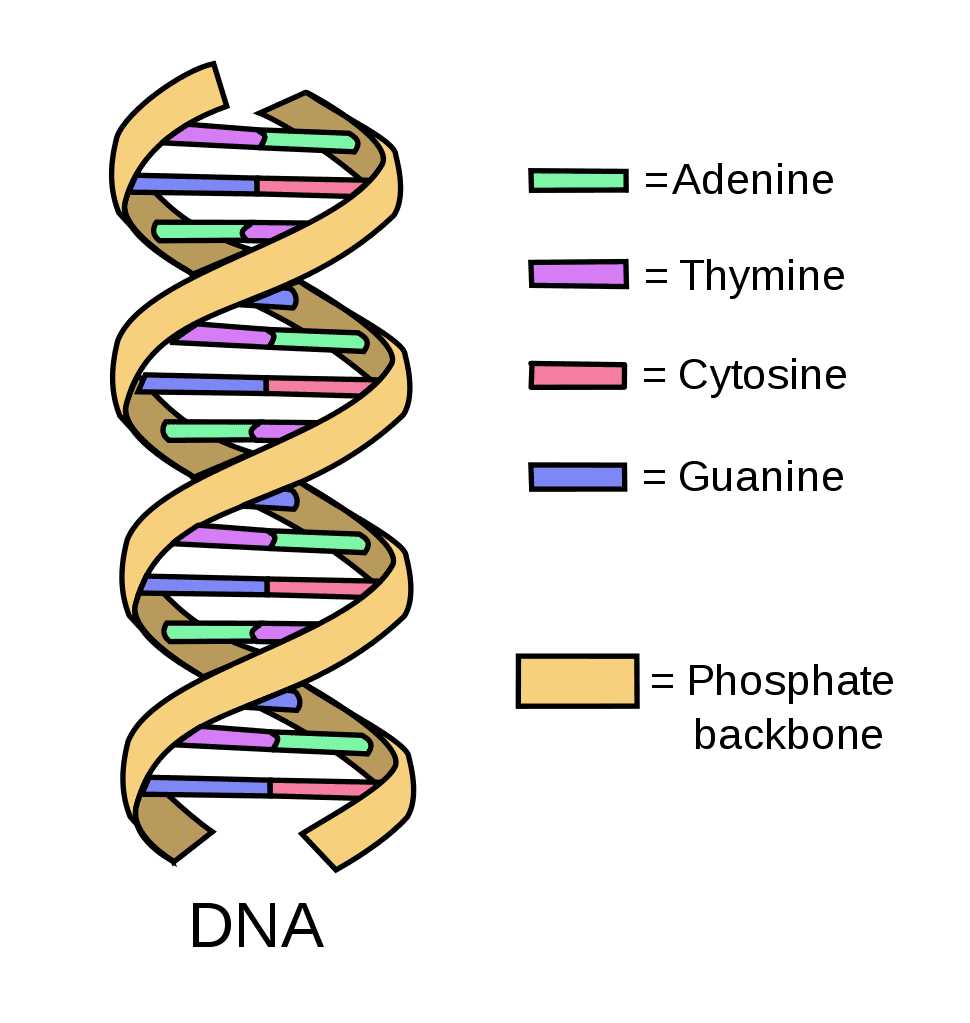
\includegraphics[width=2in]{dna}
\end{center}


\subsubsection{DNA Basics}
Deoxyribonucleic Acid, more commonly referred to as \textbf{DNA}, is the carrier of genetic information in all living beings and our storage medium of interest. A strand of DNA comprises four chemical building blocks called nucleotides which occur sequentially, connected by a sugar-phosphate backbone. The four nucleotides are also called \textbf{bases} and are named Adenine, Thymine, Guanine, and Cytosine. These are abbreviated as A, T, G, and C, respectively. Each strand has two chemically distinct ends, called 5' and 3'. A short sequence of nucleotides is commonly referred to as an \textbf{oligo}, short for oligonucleotide.

In an attempt to minimize their free energy, oligos try to bind to other oligos. This binding is done on the nucleotide level, where there are two canonical base pairings (\textbf{bps}). In these canonical base pairings, Adenine pairs with Thymine, and Guanine pairs with Cytosine. The optimal match for a DNA strand is its \textbf{reverse complement}, which is formed by interchanging each base with its canonical pairing, then reversing the sequence. Two bound, complementary strands can be referred to as \textbf{ds-DNA} (doubly stranded DNA), while a single strand can be referred to as \textbf{ss-DNA} (singly stranded DNA).

The primary structure of a DNA molecule is a double-helix, discovered by Watson and Crick in \cite{doublehelix}. In this structure, two reversely complementary strands bind to each other in a "twisted ladder" formation, where each nucleotide on one side forms a hydrogen bond with its complement.

\subsubsection{RNA}

\textbf{RNA} is another nucleic acid that primarily serves as a messenger between DNA and more functional units of an organism called proteins.

The two essential proteins we cover in this paper are \textbf{RNA-} and \textbf{DNA-polymerase}. Both act upon a region of DNA to create a copy of either itself (in the case of a DNA polymerase) or the corresponding RNA encoding (by the RNA polymerase). For our purposes, it is only relevant to regard a few aspects which set RNA apart from DNA.

\begin{itemize}
    \item Thymine is replaced with Uracil as the base-pairing for Adenine, meaning RNA consists of the bases A, U, G, and C.
    \item RNA is \textit{singly-stranded} but still often folds on itself to minimize its free energy. This folding creates secondary structures, which will be discussed in more detail later.
    \item The RNA polymerase generates RNA from a DNA strand without breaking apart the entire double helix structure at once. The molecule goes down a region of DNA like a zipper, both opening up the DNA and closing it as it travels across.
\end{itemize}

\subsubsection{Synthesis}
TODO

\subsubsection{Sequencing}
DNA's bases are read in a process called sequencing. The two most common sequencing technologies are Illumina and Nanopore sequencing. Nanopore sequencing is becoming more common, but both techniques have high error rates \cite{pcrbased}. Prices continue to drop, and the technology continues to improve, but for now, error-free sequencing is only possible with both high logical and physical redundancy.

%TODO: Write about how it is outpacing moores law%

\subsection{Biochemical Limitations Leading to Errors}
While DNA is a robust molecule when it contains biological information, one must first consider some biochemical limitations before encoding artificial data in it. This is because information encoded into living organisms has been shaped by evolution for millions of years, minimizing the following restrictions through large scale trial and error. Encoding schemes must explicitly take these limitations into account to create usable DNA storage. \\

\subsubsection{Homopolymers}
\textbf{Homopolymers} are regions of a strand that solely consist of repetitions of a single base. For example, a sequence AGCTTTTTGC contains a length five homopolymer of base T. While two to six base repeats are naturally common \cite{homopolymer}, it is crucial to avoid longer homopolymers in the encoding process, as they render a strand more error-prone \cite{homopolymererrors} and unstable. \\

\subsubsection{GC Content}
Another fundamental property of a DNA strand is its \textbf{GC Content}, which is defined as the ratio of Guanine and Cytosine bases to the rest of the bases in a region. Having a GC Content of around 50\% is essential to a strand's stability \cite{gccontent}. Still, it is not enough to calculate this ratio once over the entire strand because GC content also provides local stability. For example, a strand could have a subsequence GCGCGCGCTATATATATA with no homopolymers but a high error probability. \\


\subsubsection{Secondary Structures}
Another check to be made is for the formation of \textbf{secondary structures}. Secondary structures form when a strand binds to itself or another partially complementary strand. For example, if an ss-DNA strand contains a region of its own reverse complement, the strand can bind to itself instead of to a separate complementary strand. Such incorrect bindings cause issues when creating physical redundancy with PCR \cite{pcr} as well as at sequencing \cite{secondarystructures}. \\

%TODO: Hairpin diagram%

\subsection{DNA in storage}
A container of a solution containing ds-DNA molecules is called a \textbf{DNA pool}. Most often, all encoded data is not stored in a single container but instead divided into many DNA pools. A collection of DNA pools can be referred to as a \textbf{DNA library}. 

\subsection{Random Access}
\begin{figure}
\centering
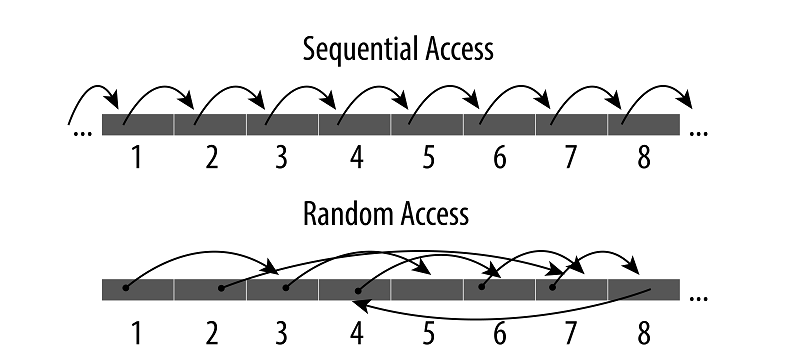
\includegraphics[width=3.5in]{randomaccess}
\caption{Random Access}
\label{randomaccess}
\end{figure}

\textbf{Random (direct) access} in a storage system is the ability to access any data fragment independently of all others. This is contrasted with sequential access, in which to access the $n$-th element, the first $n-1$ elements must have already been accessed. In order to randomly access data from a DNA library, the encoded strands and access mechanism must have the following characteristics: \\

\subsubsection{Uniquely Addressable}
Each encoded strand must have a property that allows it to be uniquely addressable independently from all other strands. \\

\subsubsection{Targetable}
For random access, one must also be capable of targeting the individual addresses of all sequences after being identified. Targeting simply means that there must be a mechanism that "searches" for a given strand independently from its neighbors in a given DNA pool. \\ 

\subsubsection{Readable}
Once the searched strand has been targeted, it must be read by some process. In the context of DNA pools, this property is given by the used sequencing technology. \\


%[1] https://www.biorxiv.org/content/10.1101/074237v3.full.pdf
%[2] https://www.sciencedirect.com/science/article/abs/pii/S0022283662801004?via%3Dihub


\subsection{Encoding Data into DNA}
In order to store data in a DNA strand, one must first consider how the data can be mapped to the four available nucleotides. This process will be referred to as encoding.

At first glance, one may try assigning each of the four bases a two-bit sequence, for example, A=00, C=01, T=10, G=11. This simple mapping would mean a byte like 01100011 would become transformed into the base sequence CTAG. However, depending on the data format, regions of the binary representation may often repeat themselves often. If one were to map two bits per base naively as described, this would result in highly error-prone strands due to excessive GC Content and long homopolymers, among other issues. For these reasons, three primary operations are performed on the data in the majority of previous work.

\subsubsection{XOR}
When encoding a library of data, it must be broken into smaller chunks because costs increase prohibitively with each added base. With each added base comes more opportunities for errors to emerge, which can propagate upwards and cause failure during amplification or sequencing.

Because digital data is non-random, i.e., much of the data we want to store is repetitive and redundant, many chunked sequences would get encoded similar to each other. If this were done without care, the sequences would not bind to their respective complementary strand but rather incompletely to neighboring similar strands. Avoiding such overlaps between sequences is what is meant by maximizing the orthogonality of the strands.

For this reason, an extra precaution is often taken as a first step, in which the bit sequence is XOR'ed with a pseudo-randomly generated sequence which can later be recovered. This procedure ensures that two similar sequences get encoded in different ways. One can consider this as a simple hashing mechanism. Of course, this pseudo-random sequence must later be regenerated to reverse this process. The reverse operation of an XOR is itself, meaning that reversing the hash is done by performing the XOR on the encoded sequence with the same pseudo-random sequence as before.

\subsubsection{Rotating Huffman Code}
One of the most obvious improvements to make at this step would be to take lessons learned from information theory into account and ensure that the encoding does not take up more bits than necessary. Not only does this reduce costs, but it also reduces the probability of errors. As stated above, much of digital data is repetitive and redundant. For this, lossless compression using Huffman coding \cite{huffmancode} as seen in \ref{code} has been used in the vast majority of recent works.

In Huffman coding, a byte sequence is separated into $n$-ary sequences, and the relative frequencies of each sequence are calculated. In our case, we use triplets of bits. A ternary tree is then generated, assigning more probable characters codes of shorter length to store data more efficiently.

This process alone, however, does not remedy the problem of repetitive regions and homopolymers. For this, a rotating code is used, which guarantees that the same base is never repeated more than once. Rotating codes entail taking the previous nucleotide into account when deciding the next base. This process is implemented with a small lookup table as depicted in TODO.

Combining these two methods allows for a sequence that fares relatively well in reducing homopolymer count and keeping GC content at around 50\%.



\begin{figure}
\centering
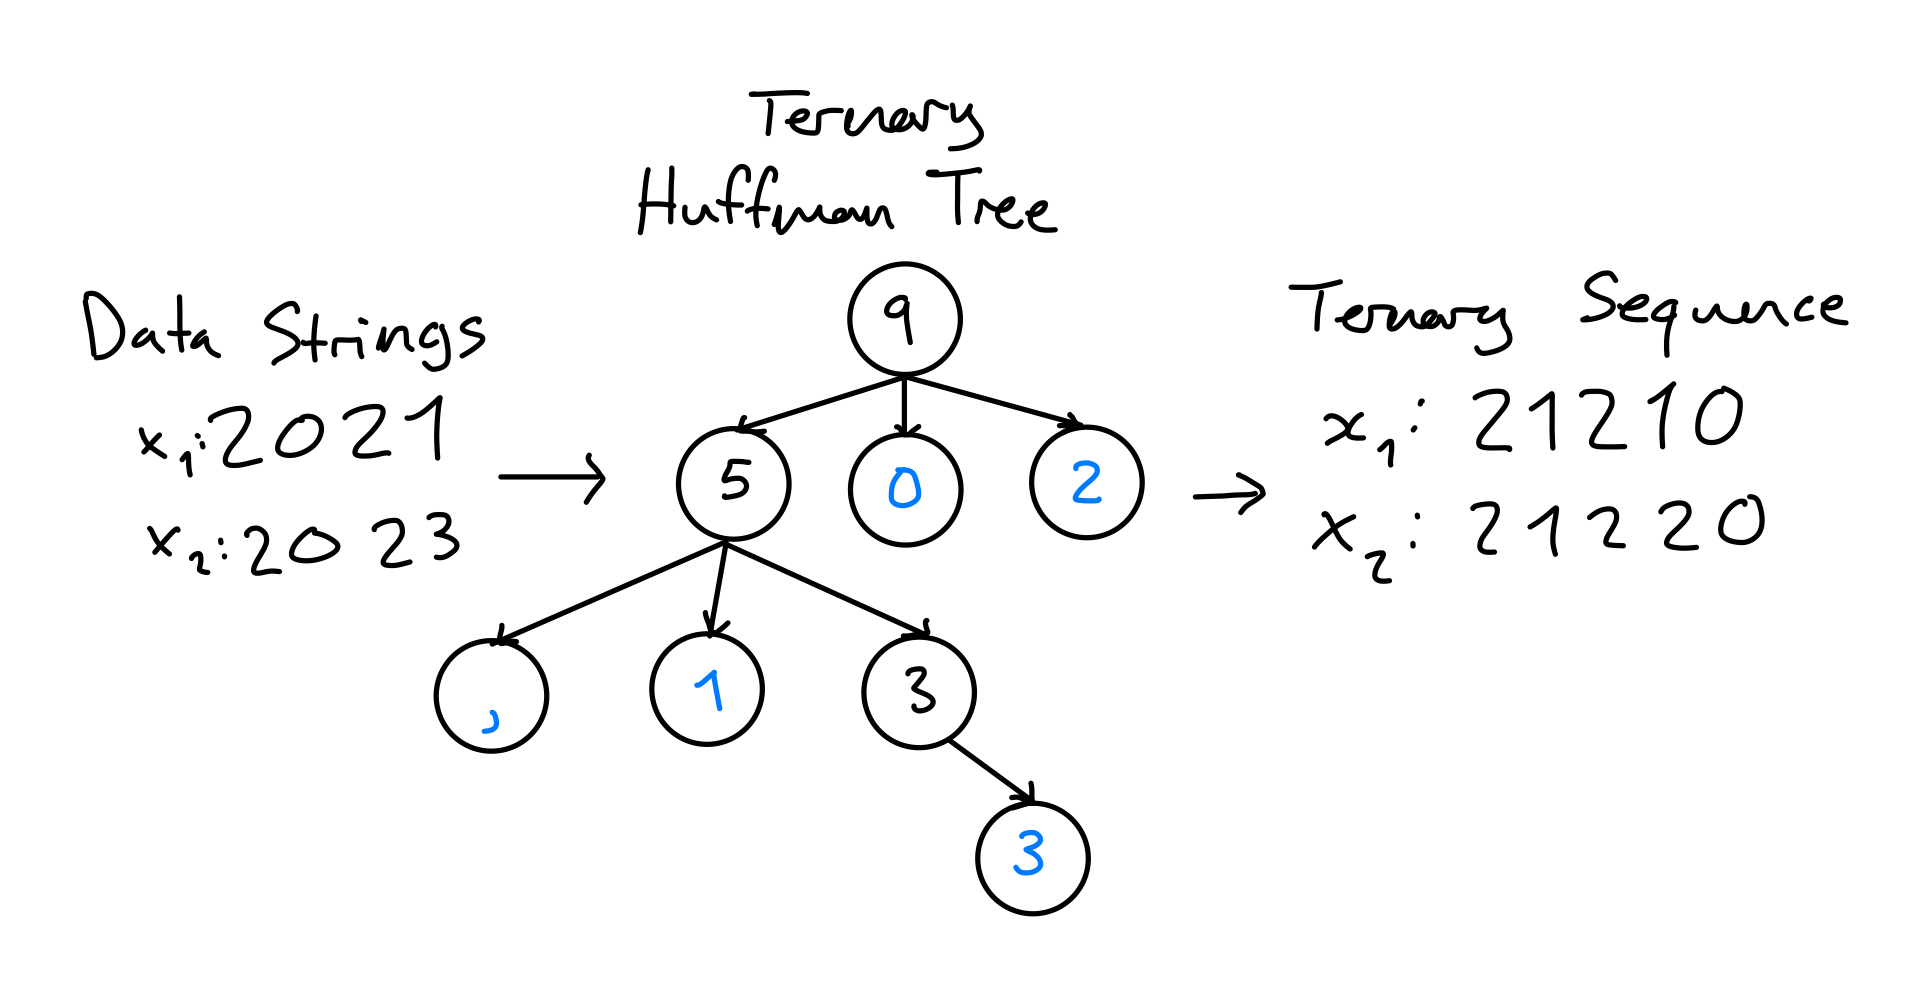
\includegraphics[width=3.5in]{huffman}
\caption{Ternary Huffman Code}
\label{code}
\end{figure}
\begin{figure}
\centering
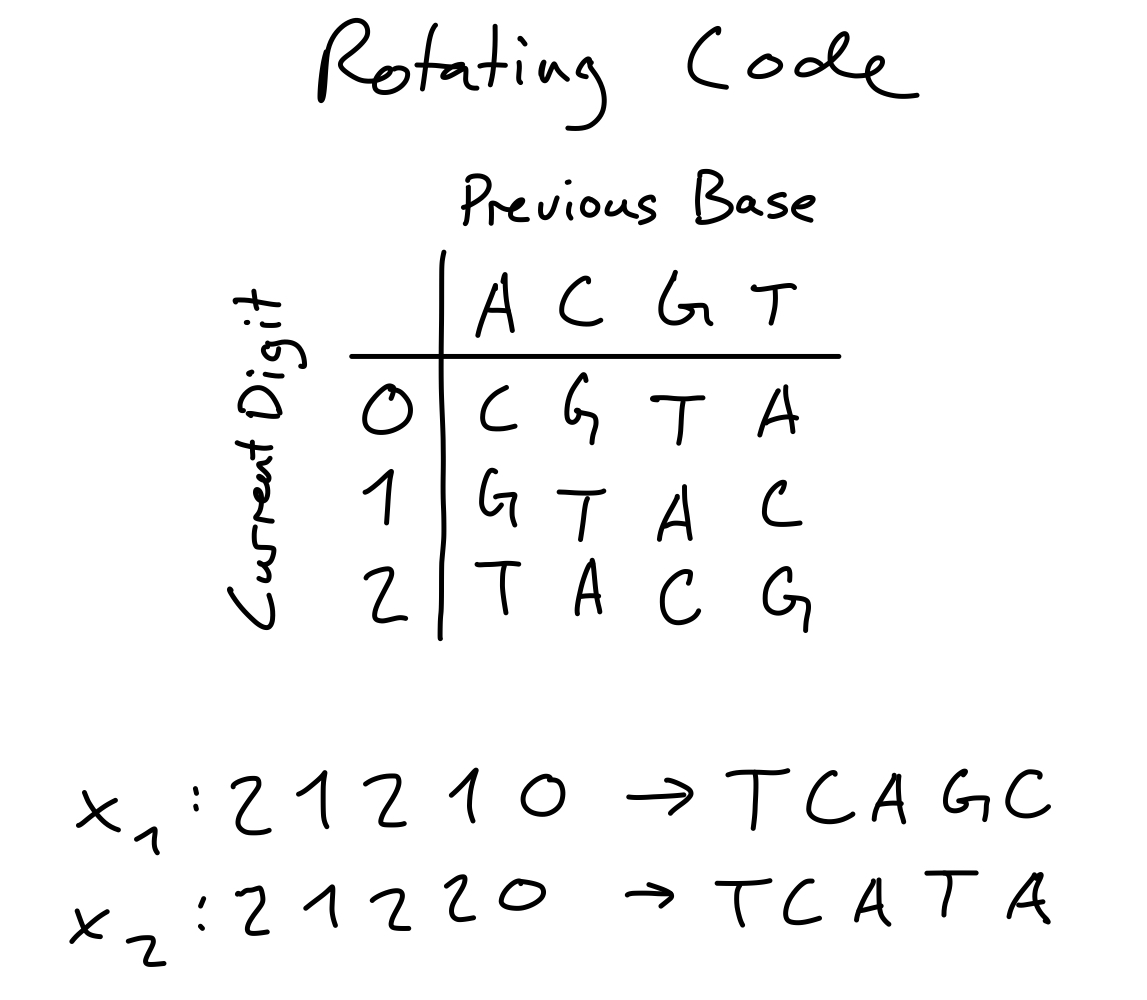
\includegraphics[width=2.5in]{rotatingcode}
\caption{Rotating Code}
\label{code}
\end{figure}

\subsection{Erasure Codes}
Due to high error rates when reading the DNA, there must be logical and physical redundancy to recover the data correctly. Physical redundancy comes from PCR discussed in the next section. The logical redundancy is commonly \cite{} implemented with erasure codes. Using an erasure code, the data sequence is transformed into a longer sequence that can be successfully decoded with only a subset of the characters from the encoding.

In current DNA libraries, the redundancy parameter is tuned relatively high \cite{pcrbased}, which significantly reduces the achieved information density. However, as sequencing technology improves, the redundancy parameter should be able to be tuned down \cite{pcrbased} due to lower read errors and improved encoding schemes which are aware of and avoid secondary structure formation and other restrictions.

In the works we will discuss the most common erasure code used is the Reed-Solomon code \cite{reedsolomoncode}. The Reed-Solomon code is a type of erasure code comprised of an inner and outer redundancy component. This technique has been widely adopted in digital systems and results in massive gains regarding the recoverability of data and the correction of errors \cite{}.



\begin{figure}[!t]
\centering
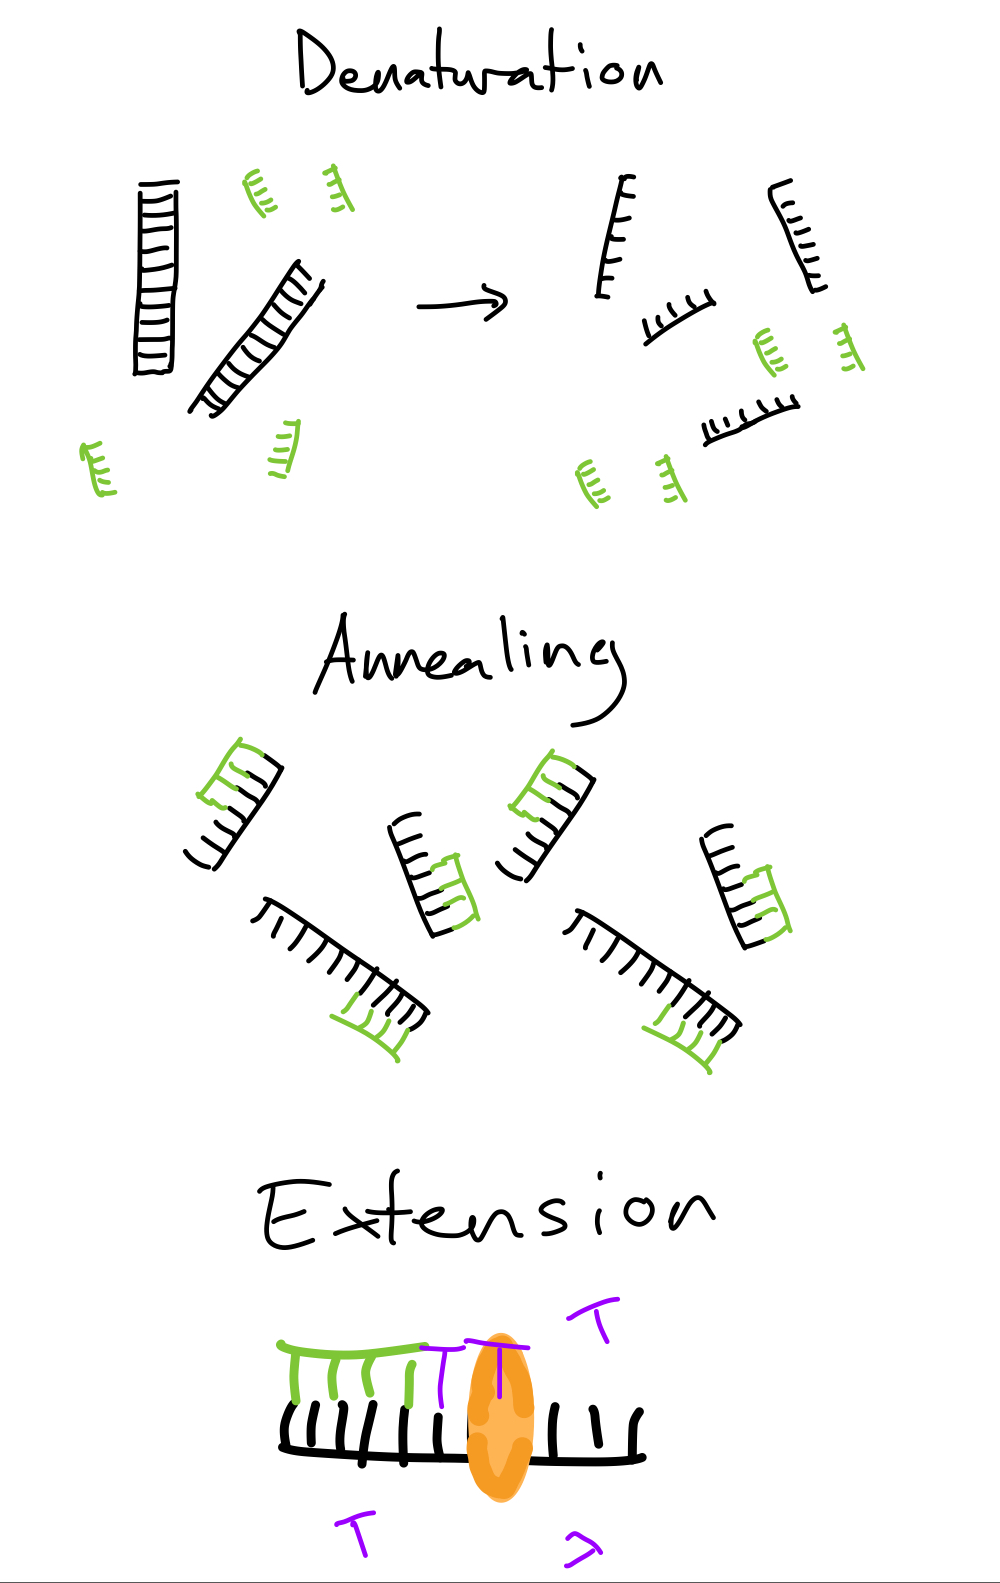
\includegraphics[width=2.5in]{pcr}
\caption{PCR Stages}
\label{fig_sim}
\end{figure}

\subsection{Introduction to PCR}

After the data has been mapped to a DNA strand, it is time to synthesize the sequences and prepare them for storage. One phase of this preparation often involves PCR (Polymerase Chain Reaction), in which each DNA sequence is multiplied millions of times. PCR is essential to create physical redundancy as well as a random access mechanism, which will be discussed in more detail later. Once data is encoded into a strand as partially described above, a so-called primer is appended to the sequence. This primer will serve as a marker of the region to be copied by an enzyme DNA polymerase. This copying, also called amplification, occurs in cycles involving the following steps. \\

\subsubsection{Denaturation}
In a process called denaturation, DNA molecules are split up into their two complementary strands by being heated to a target temperature $T_m$, called the \textit{melting point}. This melting point is determined by the temperature where 50\% of the DNA strands separate. This separation occurs because the heat breaks the hydrogen bonds holding the two strands together. This step is necessary in order to allow the complementary primer sequences to attach to each strand. \\

\subsubsection{Annealing}
Once the DNA molecules are split, the environment is cooled back down in a process called annealing. Since the strands are not bound to anything anymore, there is room for the primer sequences to bind to the complementary primer regions we appended to our data-holding DNA strand.\\

\subsubsection{Extension}
The DNA polymerase enzyme now finds the primers added in the last step and fills up the other side of the double-helix by adding free nucleotides from the solution one by one.\\

\subsubsection{Repetition}
Now that the polymerase has recreated the original double-helix, the process can cycle, restarting at the denaturation step. The number of copies doubles with each step, allowing for rapid growth.\\

\section{Current Random Access Techniques}
In the next section, we will explore three recent breakthroughs in random access for DNA storage. The main bottleneck regarding the scalability of random access to date has been the retrieval mechanism, which currently poses a much larger optimization problem than the encoding schemes. In particular, improving upon storage architectures reduces the need for high redundancy and overly robust encoding procedures, as these mainly serve to reduce the problems that the mechanism itself poses. The current available random access mechanisms heavily rely on good primer/address design, orthogonality of the encoded sequences, physical separation of the data, and the amount of data in each storage unit.


\begin{figure}[!t]
\centering
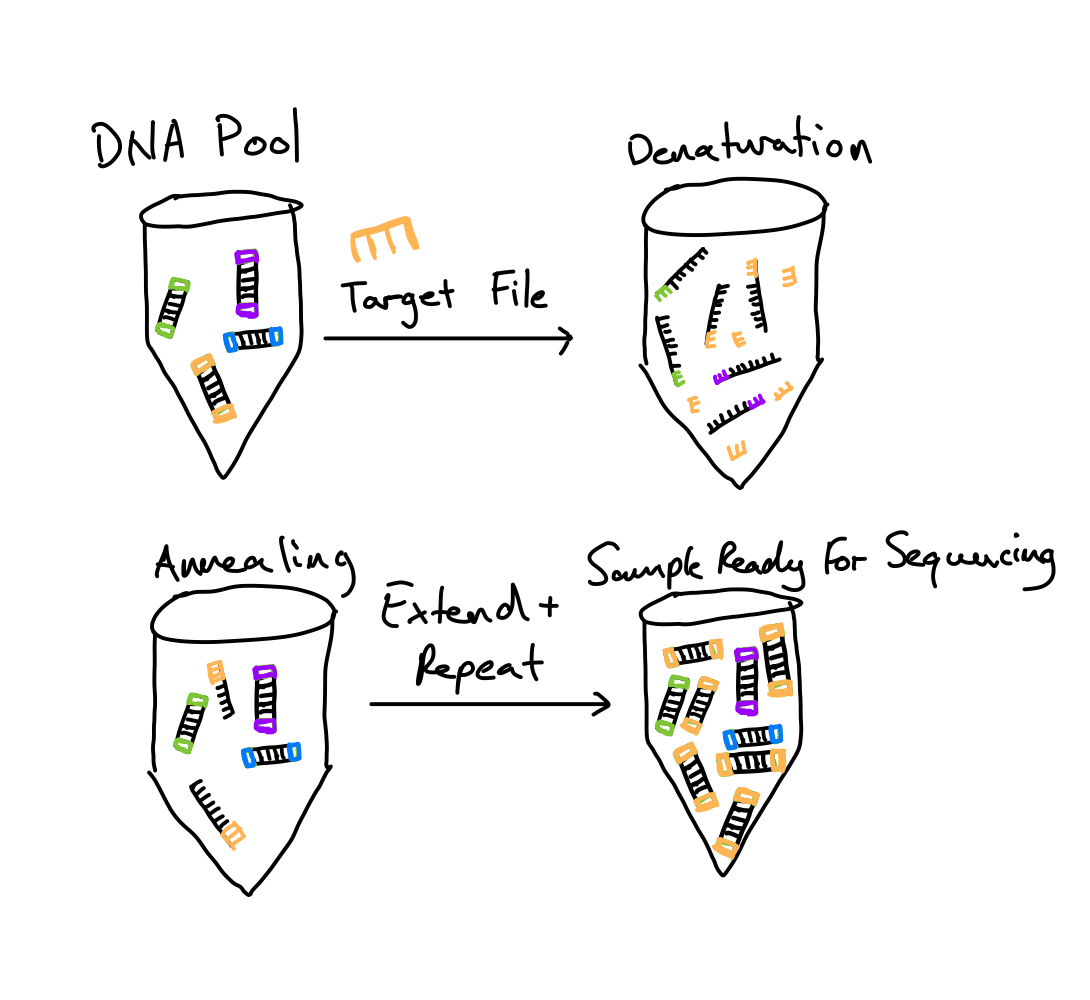
\includegraphics[width=3.5in]{pcrRA}
\caption{PCR in Random Access}
\label{fig_sim}
\end{figure}


\subsection{PCR Based Random Access}
The most basic form of random access in a DNA library can be achieved by separating files into fragments, which all receive a different PCR primer it can be identified by. Because this primer is stored in-silico, one can later re-amplify the solution containing a specific DNA fragment on retrieval. The amplification makes the sequence stand at sequencing of the DNA pool, where one sees the relative frequencies of all sequenced fragments. While this may not sound like valid random access since all data fragments are read at once, one must note that for a full read, many passes are required over the same sequence. These multiple passes are required to average out sequencing errors such as deletions, substitutions, and additions.

In addition, primer design is a delicate task, and the amount of primers that can be used is often severely limited \cite{}. As a result, most papers employ custom primer design, which is difficult, as each primer must be experimentally verified before use. This limitation is partially alleviated by breaking up a dataset into $n$ physically separated DNA pools, allowing reuse of the primers and linearly scaling direct access capability up to a certain threshold.

In previous works \cite{pcrbased} random access was performed by separating the database into $n$ DNA pools, each with a given amount $k$ of amplified DNA fragments. Each of the $k$ fragments has a unique primer used for PCR amplification, which is reused as the address to later amplify and retrieve the correct fragment. The "targetable" characteristic is given by amplifying the strand to be sequenced, effectively increasing the sequencing signal compared to the net combination of the signals from all other adjacent strands. Doing this is required because sequencing technology is indifferent to which strands we have targeted and amplified, as it will read all stands in a sample regardless. However, because the desired strand has been amplified using its primer as an address, it can be differentiated from the other sequences and decoded successfully.

Note that the scalability of this strategy depends on the number of available primers, as these can only be reused once per pool for truly individually addressable files. This is the case for various reasons. For one, as discussed above, each random access requires sequencing of the entire DNA pool since the targeted strands are not physically separated from the others. Any unamplified strands in the sample are destroyed upon sequencing, which dwindles their total supply over time. In addition, the quantity of information stored in a pool does not scale forever with the number of primers, even in cases of excellent primer design systems \cite{}. Essentially, the more sequences one adds to a pool, the more PCR cycles are needed to increase the signal of the queried strand high enough to perform a correct read. Finally, since PCR cycles involve repetitions of denaturation and annealing, any similarities between stored sequences will propagate errors due to unwanted interference through incorrect bindings and formations of secondary structures.

In \cite{pcrbased}, Organick et al. encoded and stored over 200MB of data spanning across 35 distinct files, each of which were recovered individually and without errors using PCR-based random access. The main innovation presented in their work was showing the scalability of the PCR-based random access technique and creating a new algorithm to reduce the read coverage needed at sequencing. The new algorithm made it more practical to access a file from a pool by reducing the number of needed PCR cycles to amplify the queried data. This additionally reduced the damage done to neighboring sequences. Notably, their team was the first to prove that random access could be scaled up to a library size of 200MB and theoretically much higher.

Their DNA library consisted of more than 13 million DNA oligos in total. They encoded each digital file into megabyte-sized blocks before encoding, appending the file address (PCR primer) to each block, then applying a Reed-Solomon Code. Before the data blocks were transformed to nucleotides, an outer code was applied that added new blocks to the file containing redundant information. After this, an inner code is generated and applied to each bit sequence. In this process, the bit string is translated into the encoded bases with added redundancy. 

To reduce the number of needed cycles before sequencing, they also introduced an algorithm based on bitwise majority alignment (BMA), allowing one to cluster the data from the noisy sequencing reads more efficiently. This consists of four stages which will not be discussed here. The team tested their algorithm with both Illumina sequencing and micropore sequencing technologies, although Illumina sequencing was the primary sequencing technology used for retrievals.

In \cite{pcrbased2}, Yazdi et al. implement a comparable system, except with a focus on maximizing block length to diminish read errors instead of using shorter sequence lengths with higher redundancy. Because they had longer information strings in each sequence (1000bps), they were able to reach a higher information density of $4.9 \times 10^{20}$ B/g. They argue, "Instead of storing blocks mimicking the structure and length of reads generated during high-throughput sequencing, we synthesized blocks of length 1000bps tagged at both ends by specially designed address sequences. Adding addresses to short blocks of length 100bps would incur a large storage overhead, while synthesizing blocks longer than 1000bps using current technologies is prohibitively costly."

In contrast to \cite{pcrbased}, \cite{pcrbased2} supported the rewriting of data. However, the scale of this experiment must be considered. Only six Wikipedia articles were stored, comprising in total only 17Kbs of data. This inherently lessens error rates, even considering their specially crafted encoding scheme. Therefore, these results must be replicated on a larger scale to make significant conclusions. 

\subsubsection{Limitations}
Because there are typically around a maximum of 10 primers per DNA pool \cite{}, there is a limit of $10n$ individually addressable distinct data fragments. In addition, the mapping of key-value pairs and a mapping of the file to its respective DNA pool location must be stored in-silico for later retrieval. Unfortunately, one cannot easily scale the number of primers since their design is computationally tricky. Not only this, but error rates snowball with each additional primer added to a pool since they must all be optimally orthogonal to each other in order to reduce the chance of catastrophic failure or incorrect addressing.

These limitations suggest that although PCR-based random access has scaled well as a first-generation random access system and is quite robust, it cannot scale strongly enough to compete with traditional storage mediums. This is especially the case when one considers that there needs to be a physical copy of each DNA pool, and the number of times random access to a DNA pool can be carried out is limited by the number of physical copies that exist.

A general problem caused by PCR-based random access is that its operations are destructive. Because there is no real separation of data upon reading from a pool, data that is not being addressed will be sequenced and thus destroyed upon reading. Additionally, only the directly accessed data is amplified using PCR, meaning that reads dwindle the supply of less-often accessed data. Most works using PCR-based random access use sequencing techniques that destroy the targeted sequence as well as the sequences that are not being accessed.

\subsection{Random Access using Chemical Handles}

\begin{figure}[!t]
\centering
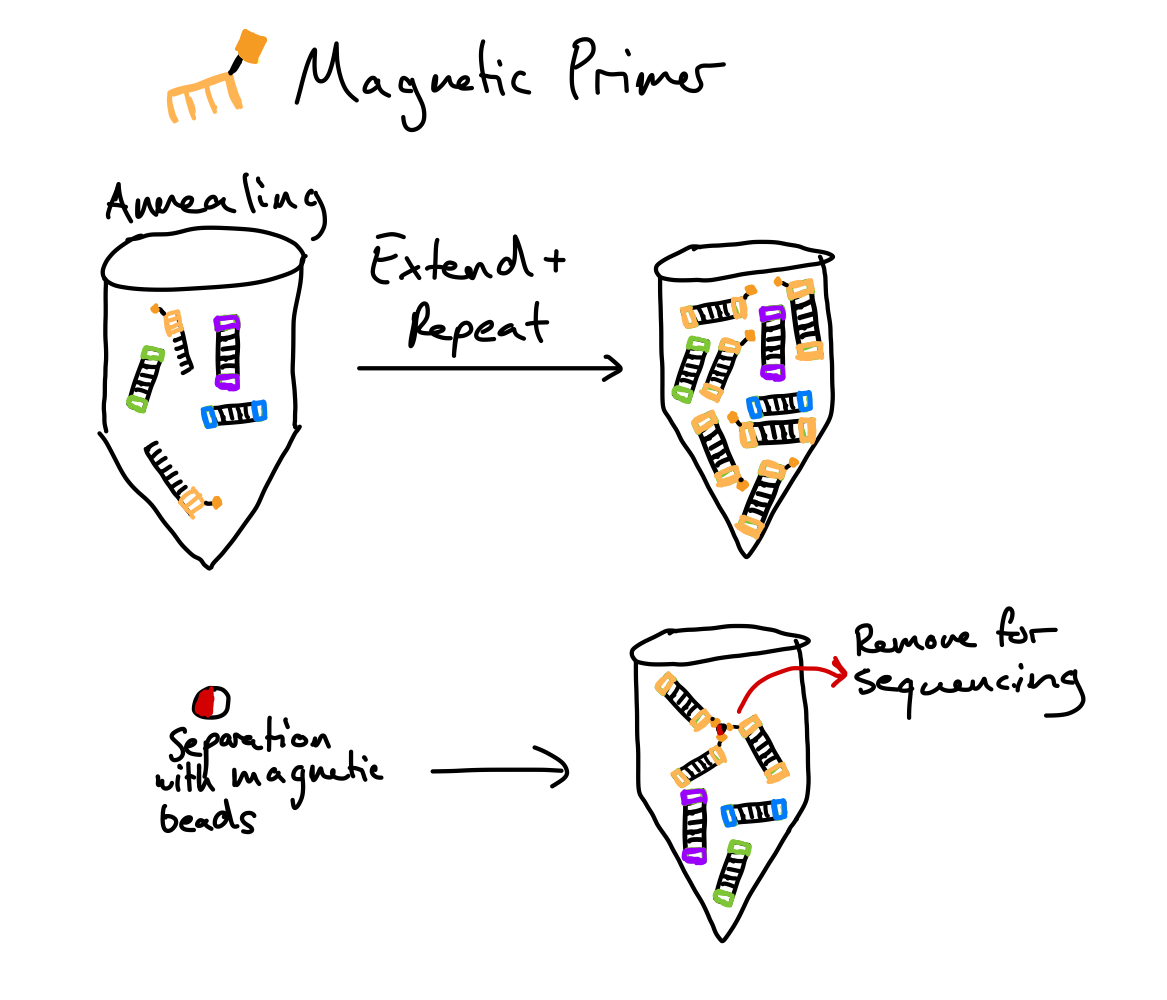
\includegraphics[width=3.5in]{chemicalHandlesRA}
\caption{Chemical Handles and Magnetic Beads}
\label{pcr_challenges}
\end{figure}

The first most considerable improvement to be made to the previously mentioned PCR approach is to isolate the identified strands physically from their neighbors before sequencing. In doing this, one can sequence the queried information independently from its neighboring strands, making analysis and sequencing more efficient while leaving the original DNA pool more or less intact.

In \cite{chemicalhandles}, Tomek et al. took on this issue inspired by \cite{chemicalhandles} work with TODO. They achieved this goal with the use of primers containing chemical handles. The primers contain identical nucleotides as before, so the main difference is that they are sequenced with a modification such that a magnetizable chemical is attached to one of the ends of the sequence. Thus, the original data pool is subjected to fewer PCR cycles upon random access, notably less than a PCR-only-based approach. Minuscule magnetic beads are then added to the sample, which attract the modified primers. These magnetic beads allow for the removal of the queried sequences so that the rest of the sequences in the original DNA pool are mainly left unaffected.

Tomek et al. also made use of nested primers. They created a system where not only one primer was used to address a sequence, but rather multiple. Each address remains unique, however, because the ordering of the primers is different for each sequence. This system increases the maximum system capacity significantly, albeit extending the header size. TODO why? These headers are generated with a hierarchical system instead of appending each other in a random permutation. The hierarchical system works as follows:  todo.

However, this specific approach only encoded five separate files, each split up into blocks of 200 bp each. Nonetheless, they also mixed in background DNA to simulate an environment of 5TB. However, these background data strands did not contain encoded information and could not simulate unwanted interaction between similar strands during PCR.

\subsection{Random Access with RNA Polymerase}
In \cite{DORIS}, Lin et al. expanded upon the chemical header architecture in a system they named DORIS (Dynamic Operations and Reusable Information Storage). Rather than using PCR primers for addresses, a custom header is instead affixed to the sequence containing a file address and a T7 promoter. This T7 promoter works analog to a PCR primer, except that it is targeted by an RNA polymerase instead of a DNA polymerase. The file address hangs off the sequence as ss-DNA and gives the "uniquely addressable" property. The targetable property is achieved through magnetic separation, as discussed beforehand. The major innovation here is that the sequences stay doubly stranded throughout the entire process. The chemically modified primers readily bind to the overhang without a denaturation and annealing process so that PCR cycles are not needed. 

The following steps are taken to access a sequence randomly. First, the complement of the hanging portion of the ss-DNA is synthesized with a chemical alteration on its 5' end to make it magnetizable. The synthesized strand is released in the DNA pool, where it binds to the overhang of the addressed sequence. After binding, all copies of the queried strand can then be isolated from the other sequences magnetically using minuscule beads, similarly to the previous approach. Next, an RNA polymerase targets the T7 promoter, where it non-destructively transcripts the sequence to RNA (in-vitro transcription). The RNA polymerase traverses the sequence, unzipping the target strand while peeking at its bases, creating a copy, subsequently re-zipping the sequence back up as it glides along. The most important takeaway here is that an RNA polymerase creates a template of a sequence without denaturation and annealing, which is a process that becomes more and more delicate as the size of the data storage in a given DNA pool increases.

The RNA is then converted back into cDNA with reverse transcription, then converted back into a double-stranded version (second-strand synthesis reaction).

The file operations are carried out in different ways, all exploiting the overhang containing the address. A significant advantage of this approach is that the doubly stranded portion of the sequences stays bound throughout the entire process, meaning that they cannot bind to other strands that would otherwise interfere with each other during PCR cycles.

Using this technique, DORIS facilitates scalable random access with non-destructive reads and additional file operations that are not supported in other works, such as locking, unlocking, renaming, and deleting. In other coding schemes, direct access is destructive because the original copies and neighboring sequences are destroyed in the sequencing process. The authors argue that these file operations are necessary steps forward in creating a realistically usable DNA storage system.

These file operations work by taking advantage of the ss-DNA overhang. For example, a rename operation takes place by synthesizing the overhang's complement appended onto a new address. The sequence becomes longer as it still contains both addresses, but only the new one is addressable since it forms the new overhang. Additionally, the double address does not affect the targeting and transcription of the sequence, as the T7 promoter is found after both addresses. A deletion can be carried out simply by releasing the complement of the overhang into the sample without a magnetic element, blocking all future accesses.

The work presented is entirely theoretical, and the actual scalability has yet to be experimentally verified. TODO how much did they experiment

\begin{figure}[!t]
\centering
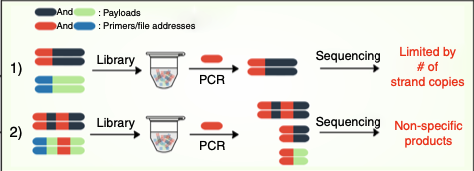
\includegraphics[width=3.5in]{pcrchallenges}
\caption{PCR Challenges}
\label{pcr_challenges}
\end{figure}

\begin{figure}[!t]
\centering
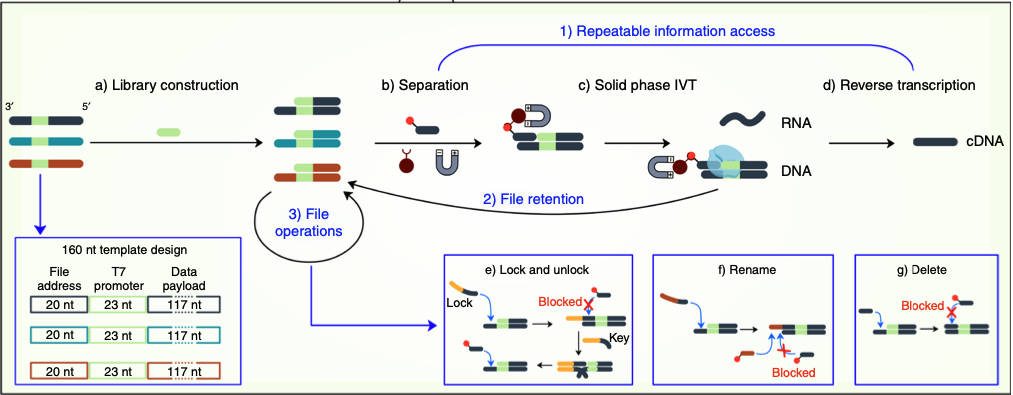
\includegraphics[width=3.5in]{doris}
\caption{DORIS}
\label{doris}
\end{figure}

\section{Comparison}
A pure PCR-based approach remains the state-of-the-art technique for random access, as it has been reproduced the most often and tested on the largest scales. However, although it has been an excellent starting point for random access, it by itself is not scalable in regards to database size and physical redundancy. 

As argued in the previous section, PCR-based random access, although robust, requires physical redundancy because each physical DNA pool can only be accessed once. Chemical handles provide a workaround by enabling the separation of the targeted strand from its neighbors before sequencing. Nonetheless, this process, as presented in \cite{chemicalhandles} still relies on PCR for amplification of the data strands. DORIS circumvents this by employing a T7 promoter, meaning that a sequence is copied with an RNA polymerase instead, leaving the original strand intact and returnable to the original DNA pool while keeping the other info sequences safe from sequencing and PCR.

The original paper using chemical handles was a theoretical breakthrough in reducing physical redundancy and providing a promising solution for reusable DNA pools. In particular, rarely accessed sequences are subjected to less stress, apart from the few PCR cycles they go through while adding the modified primers to the sample. However, this experiment was done on a small scale and could only address five different files. The same problem faces the T7 promoter-based approach, in which the authors did not disclose the amount of data used for testing. Thus, while simulations are suitable for modeling, these novel approaches must be replicated on larger scales before the approaches can be considered practically scalable. 

Nonetheless, all of these methods still rely on PCR as an addressing mechanism. Its primary goal is to target the correct strand and make it easily readable for the sequencing technology. Future techniques will need to be able to keep existing strands intact in order to maintain the re-usability of a DNA storage library. Although this is achievable in theory by chemical handles, it still is a workaround to the current sequencing technology, which gives high error rates and reads all sequences available in a given sample, regardless of what "addresses" one uses. 

%An alternative, hypothetical system which has not yet been tested could use DNA microarrays as a targeting mechanism. DNA microarrays are essentially grids of DNA binding sites, where each site contains a few (TODO) ss-DNA strands, which represent the complements of the address and primer portion of the data we want to retrieve. Combining this with promoters for RNA polymerase would mean one could safely make copies of an entire DNA library, then use microarrays to separate the sequence from its neighbors without the need for magnetic beads. 

\section{Conclusion}
As sequencing costs continue to fall and data growth rates continue to rise, DNA storage will become increasingly more attractive as time goes on. Many steps have been taken to make this a real alternative, but several factors are still to be improved upon before being considered practical (disregarding costs).

It has been shown that basic random access can be achieved using polymerase chain reaction, which continues to be the state-of-the-art method. The encoding methods used are very robust, and it can be assured with enough planning and careful encoding that each file is uniquely identifiable and directly accessible. The presented techniques for achieving random access in DNA storage libraries build on top of each other, each bringing forth new research problems to investigate in the coming years.

In particular, using chemical handles to separate the queried sequences from their neighbors physically has been experimentally tested on a small scale and provides significant re-usability of the data pool. However, it is an open question as to how this process could be optimized. One interesting facet of this optimization problem would entail investigating other primer modifications that could allow for a more straightforward extraction of the matched strands.

It has yet to be tested how the hierarchical primer approach compares to the custom address + RNA polymerase technique. In general, both mechanisms must be replicated on larger scales using actual data to shift the current paradigm.

Once the RNA polymerase technique is sufficiently experimentally verified to relieve problems posed by PCR-based random access in practice, new optimization targets can be set for further research. In particular, the viability of RNA polymerase-based approaches can be improved upon by further optimizing the re-usability of the system. This could be ameliorated by experimenting with different promoters, chemical handles, and the general methods for magnetic extraction and returning the sequences to their original DNA pool. 

One thing is clear: for large one-pot storage of information-bearing DNA strands, a PCR-based approach cannot scale. 


% trigger a \newpage just before the given reference
% number - used to balance the columns on the last page
% adjust value as needed - may need to be readjusted if
% the document is modified later
%\IEEEtriggeratref{8}
% The "triggered" command can be changed if desired:
%\IEEEtriggercmd{\enlargethispage{-5in}}

% references section

% can use a bibliography generated by BibTeX as a .bbl file
% BibTeX documentation can be easily obtained at:
% http://www.ctan.org/tex-archive/biblio/bibtex/contrib/doc/
% The IEEEtran BibTeX style support page is at:
% http://www.michaelshell.org/tex/ieeetran/bibtex/
%\bibliographystyle{IEEEtran}
% argument is your BibTeX string definitions and bibliography database(s)
%\bibliography{IEEEabrv,../bib/paper}
%
% <OR> manually copy in the resultant .bbl file
% set second argument of \begin to the number of references
% (used to reserve space for the reference number labels box)
\begin{thebibliography}{1}

\bibitem{globaldatagrowth}
Reinsel, D., Gantz, J. & Rydning, J. Data age 2025: the digitization of the world from edge to core. Idc (2018).
\bibitem{dnabasedarchival}
Bornholt, James, et al. "A DNA-based archival storage system." Proceedings of the Twenty-First International Conference on Architectural Support for Programming Languages and Operating Systems. 2016.
\bibitem{theoreticaldensity}
Church, George M., Yuan Gao, and Sriram Kosuri. "Next-generation digital information storage in DNA." Science 337.6102 (2012): 1628-1628.
\bibitem{realistictheoreticaldensity}
Wang, Y., Noor-A-Rahim, M., Zhang, J. et al. High capacity DNA data storage with variable-length Oligonucleotides using repeat accumulate code and hybrid mapping. J Biol Eng 13, 89 (2019)
\bibitem{doublehelix}
WATSON, J., CRICK, F. Molecular Structure of Nucleic Acids: A Structure for Deoxyribose Nucleic Acid. Nature 171, 737–738 (1953).
\bibitem{pcrbased}
Organick, L., Ang, S., Chen, YJ. et al. Random access in large-scale DNA data storage. Nat Biotechnol 36, 242–248 (2018).
\bibitem{DORIS}
Lin, K.N., Volkel, K., Tuck, J.M. et al. Dynamic and scalable DNA-based information storage. Nat Commun 11, 2981 (2020).
\bibitem{chemicalhandles}
Tomek, Kyle J., et al. "Driving the scalability of DNA-based information storage systems." ACS synthetic biology 8.6 (2019): 1241-1248.
\bibitem{pcrbased2}
S. M. H. T. Yazdi, Y. Yuan, J. Ma, H. Zhao, and O. Milenkovic. A Rewritable, Random-Access DNA-Based Storage System. Nature Scientific Reports, 5(14318), 2015.
\bibitem{huffmancode}
MacKay, David JC, and David JC Mac Kay. Information theory, inference and learning algorithms. Cambridge university press, 2003.
\bibitem{reedsolomoncodes}
I. S. Reed and G. Solomon. Polynomial codes over certain finite fields. Journal of the Society for Industrial and Applied Mathematics, 8(2):300–304, 1960.
\bibitem{homopolymers}
Ivády G, Madar L, Dzsudzsák E, et al. Analytical parameters and validation of homopolymer detection in a pyrosequencing-based next generation sequencing system. BMC Genomics. 2018;19(1):158. Published 2018 Feb 21. doi:10.1186/s12864-018-4544-x
\bibitem{homopolymererrors}
Shendure, Jay, and Hanlee Ji. "Next-generation DNA sequencing." Nature biotechnology 26.10 (2008)
\bibitem{pcr}
Kubista, Mikael, et al. "The real-time polymerase chain reaction." Molecular aspects of medicine 27.2-3 (2006): 95-125.
\bibitem{secondarystructures}
Dong, Fang, et al. "Secondary structure prediction and structure-specific sequence analysis of single-stranded DNA." Nucleic acids research 29.15 (2001): 3248-3257.
\bibitem{gccontent}
Yair Benita, Ronald S. Oosting, Martin C. Lok, Michael J. Wise, Ian Humphery‐Smith, Regionalized GC content of template DNA as a predictor of PCR success, Nucleic Acids Research, Volume 31, Issue 16, 15 August 2003, Page e99, https://doi.org/10.1093/nar/gng101
\end{thebibliography}




% that's all folks
\end{document}


